\documentclass[modern]{aastex62}

% Load the corTeX style definitions
% All the packages
\usepackage{url}
\usepackage{amsmath}
\usepackage{mathtools}
\usepackage{amssymb}
\usepackage{natbib}
\usepackage{graphicx}
\usepackage{calc}
\usepackage{etoolbox}
\usepackage{xspace}
\usepackage[T1]{fontenc} % https://tex.stackexchange.com/a/166791
\usepackage{textcomp}
\usepackage{ifxetex}
\ifxetex
\usepackage{fontspec}
\defaultfontfeatures{Extension = .otf}
\fi
\usepackage{fontawesome}
\usepackage{listings}
\usepackage{nicefrac}
\usepackage[bb=boondox]{mathalfa}


% Shorthand for this paper
\newcommand{\Python}{\textsf{Python}\xspace}
\newcommand{\cpp}{\textsf{C}++\xspace}
\newcommand{\bvec}[1]{{\ensuremath{\mathbf{#1}}}}
\newcommand{\xxx}[1]{{\color{red}#1}}
\DeclarePairedDelimiter\floor{\lfloor}{\rfloor}
\DeclarePairedDelimiter\ceil{\lceil}{\rceil}
\newcommand{\imag}{{\ensuremath{\mathbb{i}}}}

% References to text content
\newcommand{\documentname}{\textsl{article}}
\newcommand{\figureref}[1]{\ref{fig:#1}}
\newcommand{\Figure}[1]{Figure~\figureref{#1}}
\newcommand{\figurelabel}[1]{\label{fig:#1}}
\renewcommand{\eqref}[1]{\ref{eq:#1}}
\newcommand{\Eq}[1]{Equation~(\eqref{#1})}
\newcommand{\eq}[1]{\Eq{#1}}
\newcommand{\eqalt}[1]{Equation~\eqref{#1}}

% Add code, proof, and animation hyperlinks
\definecolor{linkcolor}{rgb}{0.1216,0.4667,0.7059}
\newcommand{\codeicon}{{\color{linkcolor}\faFileCodeO}}
\newcommand{\prooficon}{{\color{linkcolor}\faPencilSquareO}}
% !TeX root = ./ms.tex
\newcommand{\codelink}[1]{\href{https://github.com/user/repo/blob/076a0d29804b1875a480b0fd74a7ea6738368263/tex/figures/#1.py}{\codeicon}\,\,}
\newcommand{\animlink}[1]{\href{https://github.com/user/repo/blob/076a0d29804b1875a480b0fd74a7ea6738368263/tex/figures/#1.gif}{\animicon}\,\,}
\newcommand{\prooflink}[1]{\href{https://github.com/user/repo/blob/076a0d29804b1875a480b0fd74a7ea6738368263/tex/proofs/#1.ipynb}{\raisebox{-0.1em}{\prooficon}}}
\newcommand{\cilink}[1]{\href{https://dev.azure.com/user/repo/_build}{#1}}


% Define a proof environment for open source equation proofs
\newtagform{eqtag}[]{(}{)}
\newcommand{\currentlabel}{None}
\newenvironment{proof}[1]{%
\ifstrempty{#1}{%
\renewtagform{eqtag}[]{\raisebox{-0.1em}{{\color{red}\faPencilSquareO}}\,(}{)}%
}{%
\renewtagform{eqtag}[]{\prooflink{#1}\,(}{)}%
}%
\usetagform{eqtag}%
\renewcommand{\currentlabel}{#1}
\align%
}{%
\endalign%
\renewtagform{eqtag}[]{(}{)}%
\usetagform{eqtag}%
\message{<<<\currentlabel: \theequation>>>}%
}

% Define the `oscaption` command for open source figure captions
\newcommand{\oscaption}[2]{\caption{#2 \codelink{#1}}}

% Code examples
\definecolor{codegreen}{rgb}{0,0.6,0}
\definecolor{codegray}{rgb}{0.5,0.5,0.5}
\definecolor{codepurple}{rgb}{0.58,0,0.82}
\definecolor{backcolour}{rgb}{0.95,0.95,0.95}
\lstdefinestyle{mystyle}{
    backgroundcolor=\color{backcolour},
    commentstyle=\color{codegreen},
    keywordstyle=\color{magenta},
    numberstyle=\tiny\color{codegray},
    stringstyle=\color{codepurple},
    basicstyle=\small\ttfamily,
    breakatwhitespace=false,
    breaklines=true,
    captionpos=b,
    keepspaces=true,
    numbers=left,
    numbersep=5pt,
    showspaces=false,
    showstringspaces=false,
    showtabs=false,
    tabsize=2,
    aboveskip=1em,
    belowskip=1em,
    keywords=[2]{map},
    keywordstyle=[2]{\color{black!80!black}},
    upquote=true
}
\lstset{style=mystyle}

% Typography obsessions
\setlength{\parindent}{3.0ex}
\renewcommand\quad{\hskip\fontdimen3\font}



\newcommand{\s}{\bvec{s}}
\newcommand{\p}{\bvec{p}}
\newcommand{\R}{\bvec{R}}
\newcommand{\AOne}{\bvec{A_1}}
\newcommand{\alm}{\bvec{a}}
\newcommand{\Y}{\bvec{Y}}
\newcommand{\x}{\bvec{x}}
\newcommand{\kT}{\bvec{k}^\top}
\newcommand{\D}{\mathcal{D}}
\newcommand{\Doppler}{\bvec{D}}
\newcommand{\Surf}{\mathcal{S}}
\newcommand{\Curve}{\mathcal{C}}
\newcommand{\Dargs}{\bvec{d}}
\newcommand{\lmax}{\ensuremath{l_\mathrm{max}}}


% Bibliography stuff
\bibliographystyle{aasjournal}

% Begin!
\begin{document}

% Title
\title{Analytic Doppler Imaging}

% Author list
\author[0000-0002-0296-3826]{Rodrigo Luger}
\email{rluger@flatironinstitute.org}
\affil{Center~for~Computational~Astrophysics, Flatiron~Institute, New~York, NY}
%
\author{Megan Bedell}
\affil{Center~for~Computational~Astrophysics, Flatiron~Institute, New~York, NY}
%
\author{Daniel Foreman-Mackey}
\affil{Center~for~Computational~Astrophysics, Flatiron~Institute, New~York, NY}
%
\author{David W. Hogg}
\affil{Center~for~Computational~Astrophysics, Flatiron~Institute, New~York, NY}

%
\section{Introduction}
%
Check out \citet{Luger2019} and \citet{Bedell2019} and stuff.

%
\section{The problem}
\label{sec:the_problem}
%
Let $I(\lnlam, \x, t, \Dargs)$ be the specific 
intensity observed 
at log wavelength $\lnlam \equiv \ln\lambda$ and at sky-projected 
Cartesian position $\x = (x, y, z)$ on the surface of the 
star at time $t$, where
$\Dargs$ is a set of arbitrary parameters of the Doppler field.
We may express this intensity as
%
\begin{align}
    \label{eq:intro:Ixi}
    I(\lnlam, \x, t, \Dargs) &= 
        I\Big(\lnlam_0 + \D(\x, \Dargs), \x, t\Big)
\end{align}
%
where $\lnlam_0$ is the log wavelength in the rest frame and $\D$ is
the Doppler shift in log wavelength space:
%
\begin{align}
    \label{eq:intro:D}
    \D(\x, \Dargs) 
        &=
        \frac{1}{2}\ln\left( 
            \frac{1 + \beta(\x, \Dargs)}{1 - \beta(\x, 
            \Dargs)} 
        \right)
\end{align}
%
where $\beta = v(\x, \Dargs) / c$ is the ratio of the 
radial velocity at a point on the surface of the star to the speed of light.
In keeping with the literature, we take positive values of $v$ (and
$\D$) to mean redshifts.

A common approach to computing the Doppler-shifted spectrum is to
evaluate the spectrum at the rest frame wavelength $\lnlam_0$
and interpolate back to the grid in $\lnlam$. This is practical when
computing the spectrum at a single \emph{point} on the surface, but not
ideal when one is interested in the \emph{integral} over the visible
surface of the star $\Surf$, which is typically all we can observe:
%
\begin{align}
    \label{eq:intro:F}
    F(\lnlam, t, \Dargs) 
        &\equiv
        \iint\limits_{\Surf(\x)}
                I(\lnlam, \x, t, \Dargs)
        \mathrm{d}{\Surf(\x)}
        \quad ,
\end{align}
%
The difficulty in solving Equation~(\ref{eq:intro:F}) stems from the fact
that $I(\lnlam, \x, t, \Dargs)$ is difficult to write down in 
closed form, given
the non-linearity of the Doppler shift.
The standard approach to solving this integral is therefore
to discretize the surface of the star with a fine grid, evaluate the
Doppler-shifted spectrum in each cell, and sum over the spatial axes
to approximate the integral. Depending on the resolution of the grid,
this is either numerically inaccurate or computationally inefficient 
(and often both).


\section{The Solution}

\subsection{Doppler Deconvolution}

The observed spectrum is a complex function
of spatial, spectral, temporal, and velocity terms. The goal in this
section is to deconvolve each of these terms to make solving the integral
in Equation~(\ref{eq:intro:F}) easier.
%
The first thing we will do is to express Equation~(\ref{eq:intro:Ixi})
as a convolution:
%
\begin{align}
    \label{eq:deconv:convolution}
    I(\lnlam, \x, t, \Dargs) &= 
        I(\lnlam_0, \x, t) 
        * 
        \delta\big(\lnlam_0 + \D(\x, \Dargs)\big)
\end{align}
%
where $\delta$ is the
Dirac delta function and
$*$ denotes the linear convolution operator, defined for
two arbitrary functions $f$ and $h$ as the integral
%
\begin{align}
    \label{eq:deconv:convolution_def}
    (f * h)(t) \equiv \int_{-\infty}^\infty f(\tau) h(t - \tau) d\tau
\end{align}
%
for some independent coordinate $t$ and dummy parameter $\tau$.
%
The convolution of $I(\lnlam_0)$ with a delta function
has the effect of shifting the spectrum by an amount $\D$, returning
a function of the shifted (observed) log wavelength, 
$\lnlam = \lnlam_0 + \D$.

Next, we expand the spatial dependence of the
specific intensity at the rest frame wavelength
in terms of spherical harmonics on the unit disk:
%
\begin{align}
    \label{eq:deconv:Ixi0}
    I(\lnlam_0, \x, t) 
        &=
        \sum_{l=0}^\infty\sum_{m=-l}^{l} a_{lm}(\lnlam_0, t) Y_{lm}(\x)
    \quad ,
\end{align}
%
where $Y_{lm}(\x)$ is a spherical harmonic on the projected disk
and $a_{lm}(\lnlam_0, t)$ is the corresponding spherical harmonic 
coefficient at log wavelength in the rest frame $\lnlam_0$ and time $t$. For 
convenience, we may write this equation in vector form:
%
\begin{align}
    \label{eq:deconv:Ixi0vec}
    I(\lnlam_0, \x, t) &=
    \Y^\top(\x) \,
    \alm(\lnlam_0, t)
    \quad ,
\end{align}
%
where
%
\begin{align}
    \label{eq:deconv:alm}
    \alm(\lnlam_0, t) \equiv
\Big( 
    a_{0,0}(\lnlam_0, t) \quad\quad\quad\quad\quad\quad 
    a_{1,-1}(\lnlam_0, t) \quad\quad\quad\quad\quad\quad 
    a_{1,0}(\lnlam_0, t) \quad\quad\quad\quad\quad\quad
    a_{1,1}(\lnlam_0, t) \quad\quad\quad\quad\quad\quad 
    ... 
\Big)^\top
\end{align}
%
is the vector of spherical harmonic coefficients and
%
\begin{align}
    \Y^\top(\x) \equiv 
\Big( 
    Y_{0,0}(\x) \quad\quad\quad\quad\quad\quad 
    Y_{1,-1}(\x) \quad\quad\quad\quad\quad\quad 
    Y_{1,0}(\x) \quad\quad\quad\quad\quad\quad 
    Y_{1,1}(\x) \quad\quad\quad\quad\quad\quad 
    ... 
\Big)
\end{align}
%
is the corresponding vector of spherical harmonics. We may further
decompose our expression by linearizing the time dependence of the
spherical harmonic coefficients:
%
\begin{align}
    \label{eq:deconv:R}
    \alm(\lnlam_0, t) = \R(t) \alm(\lnlam_0)
    \quad ,
\end{align}
%
where $\alm(\lnlam_0) = \alm(\lnlam_0, t=t_0)$ for some reference time $t_0$.
For rigid body rotation, the result is exact and $\R(t)$ is the Wigner 
rotation matrix for real spherical harmonics 
\citep[e.g.][]{AlvarezCollado1989}, which is implicitly a 
function of the inclination, obliquity, and rotation period of the star.
In the case that other processes such as differential rotation or spot 
evolution are significant
over the course of an observation, Equation~(\ref{eq:deconv:R}) can be
made to hold approximately for some effective rotation matrix 
$\R(t)$; we discuss this later.

The equation for the specific intensity in the rest frame now reads
%
\begin{align}
    \label{eq:deconv:Ixi0vecfull}
    I(\lnlam_0, \x, t) &=
    \Y^\top(\x)
    \,
    \R(t)
    \,
    \alm(\lnlam_0)
    \quad ,
\end{align}
%
where it is clear that we have fully separated the spatial, temporal, and
spectral terms. Inserting this into Equation~(\ref{eq:deconv:convolution}) 
and integrating
over the visible portion of the star, we arrive at the expression for the 
observed spectrum:
%
%
\begin{align}
    \label{eq:deconv:F2d}
    F(\lnlam, t, \Dargs) &=
    \iint\limits_{\Surf(\x)}
    \Y^\top(\x)
    \,
    \R(t)
    \,
    \alm(\lnlam_0)
    * \delta\big(\lnlam_0 + \D(\x, \Dargs)\big)
    \mathrm{d}\Surf(\x)
    \nonumber \\[0.5em]
    &=
    \iint\limits_{\Surf(\x)}
    \Y^\top(\x)
    \delta\big(\lnlam_0 + \D(\x, \Dargs)\big)
    \mathrm{d}\Surf(\x)
    \,
    \R(t)
    \,
    *
    \,
    \alm(\lnlam_0)
    \quad ,
\end{align}
%
%
where we made use of the commutativity of the convolution operator and 
the fact that the integral is taken only over the spatial dimensions.
Note, importantly, that the convolution operation
above is implicitly a vector operation---i.e., the
convolution is taken for each spherical harmonic term individually
and then summed over all terms.

Finally, we can simplify Equation~(\ref{eq:deconv:F2d}) by noting that the
delta function in the integrand allows us to reduce the double integral 
to a line integral:
%
\begin{align}
    \label{eq:deconv:gT}
    \iint\limits_{\Surf(\x)}
    \Y^\top(\x)
    \delta\big(\lnlam_0 + \D(\x, \Dargs)\big)
    \mathrm{d}\Surf(\x)
    \, \,
    &=  
    \int\limits_{\Curve(\lnlam, \x, \Dargs)}
    \hspace*{-0.6em}\Y^\top(\x)
    \mathrm{d}\Curve(\lnlam, \x, \Dargs)
    \nonumber \\[0.5em]
    &\equiv \kT(\lnlam, \Dargs)
    \quad.
\end{align}
%
where the path $\Curve(\lnlam, \x, \Dargs)$ corresponds to the
set of all points on the visible disk where 
$\lnlam_0 + \D(\x, \Dargs) = 0$.
%
We thus have
%
\begin{align}
    \label{eq:deconv:F}
    F(\lnlam, t, \Dargs) 
    &=
    \kT(\lnlam, \Dargs) \, \R(t)
    *
    \alm(\lnlam_0)
    \quad.
\end{align}
%
Equation~(\ref{eq:deconv:F}) is the deconvolution of the
observed spectrum into velocity terms, temporal terms, and spectral/spatial
terms, respectively. In the following sections, we will discuss how to
efficiently solve the line integral in Equation~(\ref{eq:deconv:gT}).

\subsection{Computing the kernel $\kT$}
\label{sec:g}
%
In the case that the star's rotation is rigid (i.e., differential rotation
is negligible) and other effects such as convective blueshift
may be ignored, the radial velocity at any point on the surface is 
simply proportional to the distance to the axis of rotation. Without loss
of generality, if we assume the axis of rotation lies along the $y-z$ plane,
we have
%
\begin{align}
    \beta(\x, \Dargs) = \frac{\omega \sin i \, x}{c}
\end{align}
%
and
%
\begin{align}
    \label{eq:g:D}
    \D(\x, \Dargs) &= 
        \frac{1}{2}\ln\left( 
            \dfrac{1 + \dfrac{\omega \sin i \, x}{c}}
                 {1 - \dfrac{\omega \sin i \, x}{c}}
        \right)
    \quad ,
\end{align}
%
where the parameters $\Dargs$ of the Doppler field are the
angular velocity, $\omega$, and the inclination of the star with
respect to $\hat{y}$, $i$. 

In order to solve Equation~(\ref{eq:deconv:gT}), let us change basis from
spherical harmonics to polynomials on the sphere:
%
\begin{align}
    \label{eq:g:gT}
    \kT(\lnlam, \Dargs) &\equiv
    \s^\top(\lnlam, \Dargs)
    \AOne
\end{align}
%
where
%
\begin{align}
    \label{eq:g:sTdef}
    \s^\top(\lnlam, \Dargs)
    &\equiv
    \int\limits_{\Curve(\lnlam, \x, \Dargs)}
    \tilde{\p}^\top(\x)
    \mathrm{d}\Curve(\lnlam, \x, \Dargs)
\end{align}
%
is the vector of integral solutions for each spherical harmonic,
%
\begin{align}
    \tilde{\p}(\x) \equiv 
\Big( 
    1 \quad\quad\quad\quad\quad\quad 
    x \quad\quad\quad\quad\quad\quad 
    z \quad\quad\quad\quad\quad\quad 
    y \quad\quad\quad\quad\quad\quad 
    x^2 \quad\quad\quad\quad\quad\quad 
    xz \quad\quad\quad\quad\quad\quad 
    xy \quad\quad\quad\quad\quad\quad
    yz \quad\quad\quad\quad\quad\quad 
    y^2 \quad\quad\quad\quad\quad\quad
    ... 
\Big)^\top
\end{align}
%
is the polynomial basis \citep[Equation 7 in][]{Luger2019},
and $\AOne$ is the change of basis matrix from spherical harmonics
to polynomials 
\citep[Equation B11 in][]{Luger2019}. On the observer-facing surface of 
the unit sphere, the coordinate $z$ is given by $\sqrt{1 - x^2 - y^2}$.

\begin{figure}[h!]
    \begin{centering}
    \includegraphics[width=\linewidth]{figures/g.pdf}
    \oscaption{g}{%
        The Doppler $\kT$ basis for a rigidly rotating star
        computed from Equation~(\ref{eq:g:gT}) and
        Equation~(\ref{eq:g:sTrecurrence}) up to spherical 
        harmonic degree $l=10$. Rows correspond to the degree $l$ and
        columns correspond to the order $m$. These functions encode
        the contribution of each spherical harmonic to the rotational
        broadening of features in the stellar spectrum. Because the
        rotational axis is chosen to be aligned with $\hat{y}$,
        none of the $m < 0$ harmonics contribute to the observed
        spectrum.
        \label{fig:g}
    }
    \end{centering}
\end{figure}

If we assume the star is unocculted, the region of integration $\Surf$ 
is simply the unit disk, so $\Curve(\lnlam, \x, \Dargs)$ 
is the set of all points
that satisfy both $\lnlam_0 + \D(\x, \Dargs) = 0$ and 
$x^2 + y^2 \le 1$.
Solving Equation~(\ref{eq:g:D}) for $x$, we find that 
the curves $\Curve(\lnlam, \x, \Dargs)$ 
are simply vertical lines on the unit disk given by 
%
\begin{align}
    x &= 
        \Bigg(\frac{c}{\omega\sin i}\Bigg) 
        \Bigg(\frac{\mathrm{e}^{-2{\lnlam_0}} - 1}
                   {\mathrm{e}^{-2{\lnlam_0}} + 1}\Bigg)
    \quad .
\end{align}
%
The integral in Equation~(\ref{eq:g:sTdef}) is therefore just an integral
over $y$:
%
\begin{align}
    \label{eq:g:sT}
    \s^\top(\lnlam, \Dargs) 
    &=    
    \int\limits_{-\sqrt{1 - x^2}}^
                {\sqrt{1 - x^2}}
    \tilde{\p}^\top
    \Big(x, y\Big)
    \mathrm{d}y
    \quad .
\end{align}
%
From \citet{Luger2019}, the $n^\mathrm{th}$ term of the polynomial basis
is a polynomial in $x$, $y$, and $z = \sqrt{1 - x^2 - y^2}$:
%
\begin{proof}{PolynomialBasis}
    \tilde{p}_n 
    &=
    x^i y^j z^k
\end{proof}
%
where $i, j, k$ are integers given by
%
\begin{proof}{PolynomialBasis}
    \label{eq:g:lm}
    i &= \floor*{\Lambda - \Delta}
    \nonumber \\[0.5em]
    j &= \floor*{\Delta}
    \nonumber \\[0.5em]
    k &= \ceil*{\Delta} - \floor*{\Delta}
\end{proof}
%
with
%
\begin{proof}{PolynomialBasis}
    \Lambda &= \floor*{\sqrt{n}}
    \nonumber \\[0.5em]
    \Delta &= \frac{n - \Lambda^2}{2}
    \quad .
\end{proof}
%
We may now explicitly write down the $n^\mathrm{th}$ term of 
Equation~(\ref{eq:g:sT}),
%
\begin{align}
    \label{eq:g:sTexpression}
    s_n(\lnlam, \Dargs) 
    &=    
    s_{i,\,j,\,k}(\lnlam, \Dargs) 
    =    
    x^i
    \int\limits_{-\sqrt{1 - x^2}}^
                {\sqrt{1 - x^2}}
        y^j
        \left(1 - x^2 - y^2\right)^{\frac{k}{2}} \,
    \mathrm{d}y 
    \quad .
\end{align}
%
As we show in the Appendix, the solution to this integral
is analytic and expressible in terms of simple recurrence
relations. Given the boundary conditions
%
\begin{align}
    s_{0,\,0,\,0} &= 2 \sqrt{1-x^2} \nonumber \\
    s_{0,\,0,\,1} &= \frac{\pi}{2} \big(1-x^2\big) \nonumber \\
    s_{0,\,1,\,k} &= 0 \quad ,
\end{align}
%
we may compute any term in the series via the expressions
%
\begin{align}
    \label{eq:g:sTrecurrence}
    s_{0,\,j,\,k} &= \frac{j - 1}{j + 1 + k} \big(1 - x^2\big) s_{0,\,j-2,\,k} \nonumber \\
    s_{i,\,j,\,k} &= x \, s_{i-1,\,j,\,k} \quad.
\end{align}
%
Figure~\ref{fig:g} shows the $\kT$ basis computed from
the formulae above and Equation~(\ref{eq:g:gT}) up to spherical 
harmonic degree $l=10$.

This completes our derivation of the analytic expression for the
observed spectrum (Equation~\ref{eq:deconv:F}). As we show later,
this equation allows us to compute the forward model for the
spectrum very efficiently, particularly if we make use of Fast-Fourier
Transform (FFT) -based convolution techniques. However, a convolution
can also be represented as a matrix dot product, which we can use to
express the model for the observed spectrum as a purely linear
operation on the map decomposition $\alm(\lnlam_0)$. In the following section
we derive this expression and show how it can be used to obtain
fast, analytic solutions to the Doppler problem.

\subsection{Linearization}
\label{sec:linear}

\begin{figure}[ht!]
    \begin{centering}
    \includegraphics[width=0.8\linewidth]{figures/linalg.pdf}
    \oscaption{linalg}{%
        The Doppler design matrix $\Doppler$ (Equation~\ref{eq:linear:f}), 
        constructed from a grid of Toeplitz
        matrices, each of shape $K \times K'$, where $K$
        is the number of wavelength bins in the observed spectrum and
        $K' = K + W - 1$ is the number of bins in the model spectrum,
        where $W$ is the width of the convolution kernel.
        The $N$ columns of $\Doppler$ correspond
        to the Toeplitz matrices for each of the $N$ spherical harmonics
        (shown at the top);
        the $M$ rows correspond to the Toeplitz matrices rotated to each
        of the $M$ stellar phases observed (indicated graphically 
        to the left of $\Doppler$).
        \label{fig:linalg}
    }
    \end{centering}
\end{figure}

Although the convolution operator (Equation~\ref{eq:deconv:convolution_def})
is defined for continuous functions, the problem of Doppler imaging deals with
discrete measurements of a spectrum in bins of log wavelength. Provided our
wavelength grid is fine enough, we may therefore approximate 
Equation~(\ref{eq:deconv:convolution_def}) with a discrete convolution.
For discrete arrays $\bvec{f}$ and $\bvec{h}$, we have
%
\begin{align}
    \label{eq:linear:convolution_def}
    \bvec{f} * \bvec{h} = \bvec{T}(\bvec{f}) \, \bvec{h}
\end{align}
%
where $\bvec{T}(\bvec{f})$ is a Toeplitz matrix, a matrix whose diagonals
are constant from top left to bottom right. In this case, the diagonals
are constructed from the values of $\bvec{f}$. If $\bvec{f}$ has length
$N$, element $f_n$ is placed everywhere along the $k^\mathrm{th}$ diagonal 
of $\bvec{T}$ for $k = -N / 2 + n$; all other entries of $\bvec{T}$ are 
set to zero.

Given this formulation, we may re-write Equation~(\ref{eq:deconv:F}) as a
purely linear operation on $\alm(\lnlam_0)$:
%
\begin{align}
    \label{eq:linear:f}
    \bvec{f}
    &=
    \Doppler(\kT, \R)
    \,
    \alm
    \quad,
\end{align}
%
where we introduce the $(K \times N K')$ Doppler design matrix $\Doppler$, 
constructed
by concatenating the Toeplitz matrices for each of the $N$ components of the
convolution kernel $\kT(\lnlam, \Dargs)$ after rotating it (via $\R(t)$) 
to the correct stellar phase. 
%
The $(K \times 1)$ vector $\mathbf{f}$ is the model for 
the flux observed at each wavelength at a particular time, and the 
$(N K' \times 1)$ vector $\alm$ is the vector representation of the
spatially-dependent spectrum of the star. The latter is constructed
by concatenating the ...
(Equation~\ref{eq:deconv:alm})



In Figure~\ref{fig:linalg} we show an
example of $\Doppler$.


\section{Validation}
\label{sec:validation}

Words here. Figure~\ref{fig:spot} and Figure~\ref{fig:compare}.

\begin{figure}[p!]
    \begin{centering}
    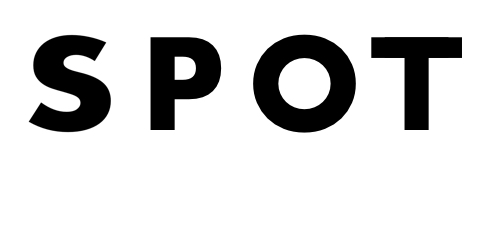
\includegraphics[width=0.6\linewidth]{figures/spot.pdf}
    \oscaption{spot}{%
        Time evolution of a Gaussian absorption line on a rigidly rotating, 
        spotted star computed from the analytic formulae in \S\ref{sec:g}.
        The stellar surface is modeled as a spherical harmonic expansion
        up to $l=20$, and the line shape is assumed to be the same everywhere;
        the spot simply downweights the local intensity at all wavelengths.
        As the spot rotates into view (left panel), the line shape changes
        slightly (center panel). The residuals between the line when the
        spot is in view (solid) and when it is on the backside of the star
        (dotted) are shown in the right panel, where
        a Gaussian-like feature can be seen tracking the spot as it rotates
        from the blueshifted hemisphere to the redshifted hemisphere of
        the star.
        \label{fig:spot}
    }
    \end{centering}
\end{figure}

\begin{figure}[h!]
    \begin{centering}
    \includegraphics[width=0.65\linewidth]{figures/compare.pdf}
    \oscaption{compare}{%
        The observed spectrum when the spot is in view computed with
        \starry (blue) and numerically (orange). The problem setup
        is the same as that in Figure~\ref{fig:spot}. The bottom
        panel shows the absolute value of the difference between the 
        two spectra for different grid resolutions in the numerical solution.
        As the number of grid points increases, the numerical solution
        approaches the \starry solution.
        \label{fig:compare}
    }
    \end{centering}
\end{figure}


\section{Performance}
\label{sec:performance}

Evaluation of the model via Equation~(\ref{eq:deconv:F}) requires 
first the rotation of the $(\lmax + 1)^2$
$\kT$ kernels (each of length $W$) to the correct stellar 
rotational phase, an operation that scales approximately
as $W \lmax^3$,
followed by $(\lmax + 1)^2$
linear convolutions of the rotated $\kT$ kernels with the 
spectral components (each of length $K$), which scales
approximately as $W K \lmax^2$. Since typically $K \gg \lmax$,
the latter computation dominates and the entire evaluation 
takes $\mathcal{O}(W K \lmax^2)$ operations.




%
%
%
%
\clearpage
\appendix
%
%
%
%

\section{Integrals}
\subsection{Equation~(\ref{eq:g:sTexpression})}
%
In this section we derive the recurrence relations
(\ref{eq:g:sTrecurrence}) for computing $\s^\top$.
When $i = k = 0$, the integral is easy to evaluate:
%
\begin{align}
    s_{i,\,j,\,0}(\lnlam_0) 
    &=    
    \begin{cases}
        2 \left( 1 - x^2 \right)^\frac{j + 1}{2} 
        \quad\quad\quad\quad\quad\quad\quad\quad\quad\quad\quad\quad 
        &  j \, \mathrm{even} \\
        0 & j \, \mathrm{odd} \quad .
    \end{cases}
\end{align}
%
The general term may be computed from the recurrence relation
%
\begin{align}
    s_{0,\,j,\,0}(\lnlam_0) = \frac{j - 1}{j + 1} \big(1 - x^2\big) s_{0,\,j-2,\,0}
\end{align}
%
provided 
%
\begin{align}
    s_{0,\,0,\,0} &= 2 \sqrt{1-x^2} \nonumber \\
    s_{0,\,1,\,0} &= 0 \quad.
\end{align}
%
When $i = 0$ and $k = 1$, we may substitute $y = \sin\psi\sqrt{1 - x^2}$ in
the integrand to obtain
%
\begin{align}
    s_{0,\,j,\,1}(\lnlam_0)
    &=
    (1 - x^2)^{\frac{j + 2}{2}}
    \int\limits_{-\frac{\pi}{2}}^{\frac{\pi}{2}}
        \sin^j\psi
        \cos^2\psi \,
    \mathrm{d}\psi
    \quad.
\end{align}
%
We may solve this integral using the recurrence relation
%
\begin{align}
    \int
        \sin^j\psi
        \cos^m\psi \,
    \mathrm{d}\psi
    &=
    -\frac{\sin^{j-1}\psi \cos^{m+1}\psi}{j + m}
    +
    \frac{j - 1}{j + m}\int\sin^{j-2}\psi \cos^m\psi \mathrm{d}\psi
    \quad ,
\end{align}
%
which, in our case, simplifies to
%
\begin{align}
    \int\limits_{-\frac{\pi}{2}}^{\frac{\pi}{2}}
        \sin^j\psi
        \cos^2\psi \,
    \mathrm{d}\psi
    &=
    \frac{j - 1}{j + 2}\int\limits_{-\frac{\pi}{2}}^
        {\frac{\pi}{2}}\sin^{j-2}\psi \cos^2\psi \mathrm{d}\psi
    \quad.
\end{align}
%
We thus arrive at the recurrence relation
%
\begin{align}
    s_{0,\,j,\,1} &= \frac{j - 1}{j + 2} \big(1 - x^2\big) s_{0,\,j-2,\,1}
\end{align}
%
with initial conditions
%
\begin{align}
    s_{0,\,0,\,1} &= \frac{\pi}{2} \big(1-x^2\big) \nonumber \\
    s_{0,\,1,\,1} &= 0 \quad.
\end{align}
%
Given these expressions, recursing upward in $i$ is easy:
%
\begin{align}
    s_{i,\,j,\,k} &= x \, s_{i-1,\,j,\,k} \quad.
\end{align}

% Bibliography
\bibliography{bib}

\end{document}
